%This work is licensed under the Creative Commons License Attribution 4.0 International (CC-BY 4.0)
%https://creativecommons.org/licenses/by/4.0/legalcode
\documentclass[rgb]{standalone}
\usepackage{tkz-euclide}
\definecolor{myorange}{hsb}{0.0833, 1, 0.8}
\definecolor{mygreen}{hsb}{0.3333, 1, 0.8}
\definecolor{myblue}{hsb}{0.5833, 1, 0.8}
\definecolor{mymagenta}{hsb}{0.8333, 1, 0.8}
\begin{document}
	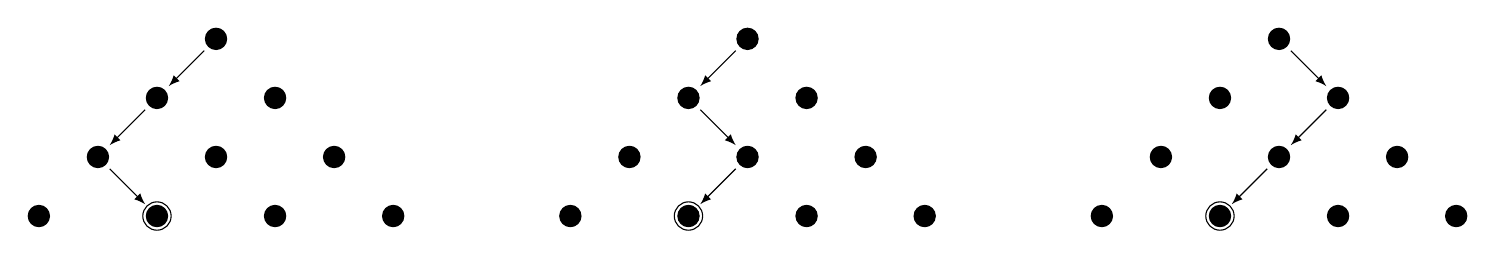
\begin{tikzpicture}[scale=1.5, font=\Large]
		\foreach \i in {0,...,3} {
			\foreach \j in {0,...,\i} {
				\filldraw (1*\j-0.5*\i,-0.5*\i) circle [radius=0.09cm];
				\filldraw (1*\j-0.5*\i+4.5,-0.5*\i) circle [radius=0.09cm];
				\filldraw (1*\j-0.5*\i+9,-0.5*\i) circle [radius=0.09cm];
			}
		}
	\draw[-latex] (-0.1,-0.1) -- (-0.4,-0.4);
	\draw[-latex] (-0.6,-0.6) -- (-0.9,-0.9);
	\draw[-latex] (-0.9,-1.1) -- (-0.6,-1.4);
	\draw[-latex] (4.4,-0.1) -- (4.1,-0.4);
	\draw[-latex] (4.1,-0.6) -- (4.4,-0.9);
	\draw[-latex] (4.4,-1.1) -- (4.1,-1.4);
	\draw[-latex] (9.1,-0.1) -- (9.4,-0.4);
	\draw[-latex] (9.4,-0.6) -- (9.1,-0.9);
	\draw[-latex] (8.9,-1.1) -- (8.6,-1.4);
	\draw (-0.5,-1.5) circle [radius=0.12cm];
	\draw (4,-1.5) circle [radius=0.12cm];
	\draw (8.5,-1.5) circle [radius=0.12cm];
	\end{tikzpicture}
\end{document}